\documentclass[letterpaper]{article}

\usepackage[utf8]{inputenc}
\usepackage{microtype}
\usepackage[usenames,dvipsnames,svgnames]{xcolor}
\usepackage{menukeys}
\usepackage{subcaption}

\usepackage{listings}
\lstset{
    basicstyle=\scriptsize\ttfamily,
    commentstyle=\color{Gray},
    extendedchars=true,              % lets you use non-ASCII characters; for 8-bits encodings only, does not work with UTF-8
    frame=single,                    % adds a frame around the code
    keepspaces=true,                 % keeps spaces in text, useful for keeping indentation of code (possibly needs columns=flexible)
    keywordstyle=\color{BurntOrange},
    language=C++,
    otherkeywords={void, Servo},
    numbers=left,
    numbersep=5pt,
    numberstyle=\scriptsize,
    rulecolor=\color{black},
    showspaces=false,
    showstringspaces=false,
    showtabs=false,
    stringstyle=\color{Blue},
    tabsize=2
}

\usepackage{graphicx}
\graphicspath{ {img/} }

\title{Build Your First Robot with Arduino}
\author{UW Tacoma IEEE Student Branch}

\begin{document}

\maketitle

An Arduino is an open-source physical computing platform.
That means its a way to program \emph{things}.
You can use an Arduino to control lights, motors, buttons, or almost anything.
Arduinos provide a beginner friendly way to program microcontrollers.
We'll be using the Arduino Uno,
the most standard Arduino model.

\begin{figure}[h!]
    \centering
    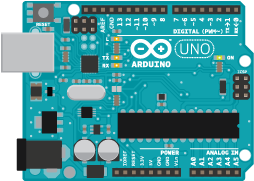
\includegraphics[width=.5\textwidth]{uno.png}
    \caption{Arduino Uno}
\end{figure}

\section{Getting Started}
\label{sec:getting_started}

To program the Arduino,
we'll use the Arduino IDE (integrated development environment).
Open the start menu and type ``arduino'' to find it.
It should look something like Figure~\ref{fig:ide}.
This is the application we'll use to write code
and upload it to the Arduino board.

\begin{figure}[h!]
    \centering
    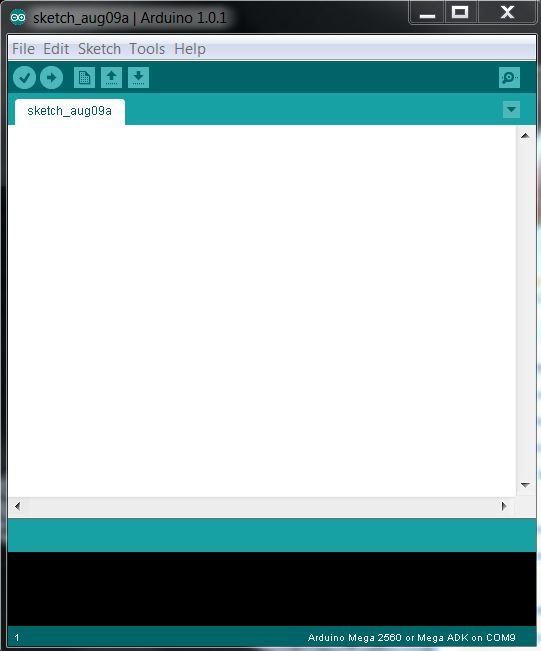
\includegraphics[width=.5\textwidth]{ide.jpg}
    \caption{Arduino IDE}
    \label{fig:ide}
\end{figure}

We'll start by blinking a light with our Arduino.
Select \menu{File>Examples>>01.Basics>Blink}.
This will load the code for a program that blinks a light.

Next we put the code onto the board.
Select \menu{Tools>Board>Arduino Uno}.
This tells the program which type of board we're using.
Plug the board into your computer with a USB cable.
Go to \menu{Tools>Port} and make sure something is checked.
This tells the computer where to find your Arduino.
Finally, select \menu{File>Upload}.
A progress bar will show you as the code is sent to the board.

Congratulations!
You have just programmed your Arduino.
You should see the LED (light emitting diode) on your board blinking.

\section{Building Your Robot}
\label{sec:wiring_your_robot}

Before we program our robot, we have to build it.
We'll use two servo motors to move.
A servo is a precisely controlled motor (see Figure~\ref{fig:servo}).
A servo has three wires to connect as shown in Figure~\ref{fig:connector}.
The black and red wires are for power.
Black is connected to \emph{ground} which means zero volts.
Red is connected to 5 volts.
The white wire is for \emph{signal}.
This is what we use to tell the servo how to turn.

Servos use \emph{pulse width modulation} (PWM).
PWM is a special kind of signal from the Arduino.
The Arduino can only make this signals on pins
labeled with a `\texttt{\textasciitilde}'.
We'll use pin 10 for the right servo
and pin 11 for the left servo.

\begin{figure}[h!]
    \centering
    \begin{subfigure}[b]{.45\textwidth}
        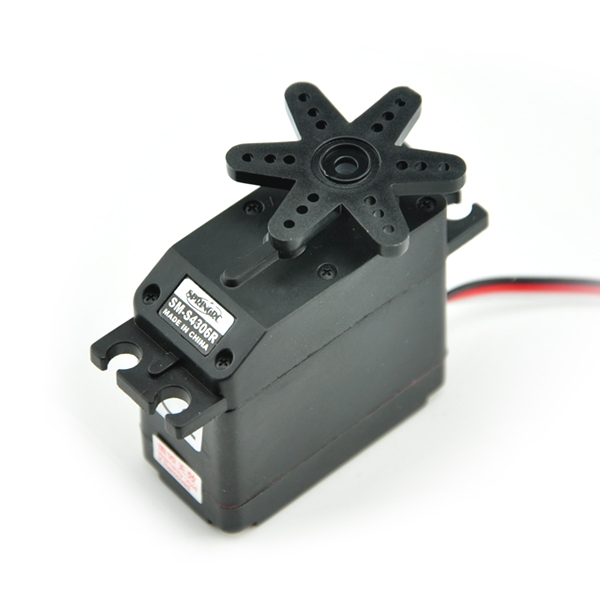
\includegraphics[width=\textwidth]{servo.jpg}
        \caption{servo motor}
        \label{fig:servo}
    \end{subfigure}
    ~
    \begin{subfigure}[b]{.45\textwidth}
        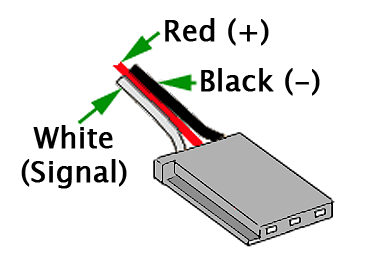
\includegraphics[width=\textwidth]{connector.png}
        \caption{servo connector}
        \label{fig:connector}
    \end{subfigure}
    \caption{}
\end{figure}

Figure~\ref{fig:circuit} shows all the connections we need to make.
Use jumper wires to make these connections:
\begin{enumerate}
    \item Right servo ground (black) to Arduino ground (GND)
    \item Left servo ground (black) to Arduino ground (GND)
    \item Right servo signal (white) to Arduino pin 10
    \item Left servo signal (white) to Arduino pin 11
    \item Right servo high (red) to Arduino 4 volt (5V) to left servo high (red)
\end{enumerate}
Since there is only one 5V pin on the Arduino,
we'll use a Y-jumper cable with and extra connection point.

\begin{figure}[h!]
    \centering
    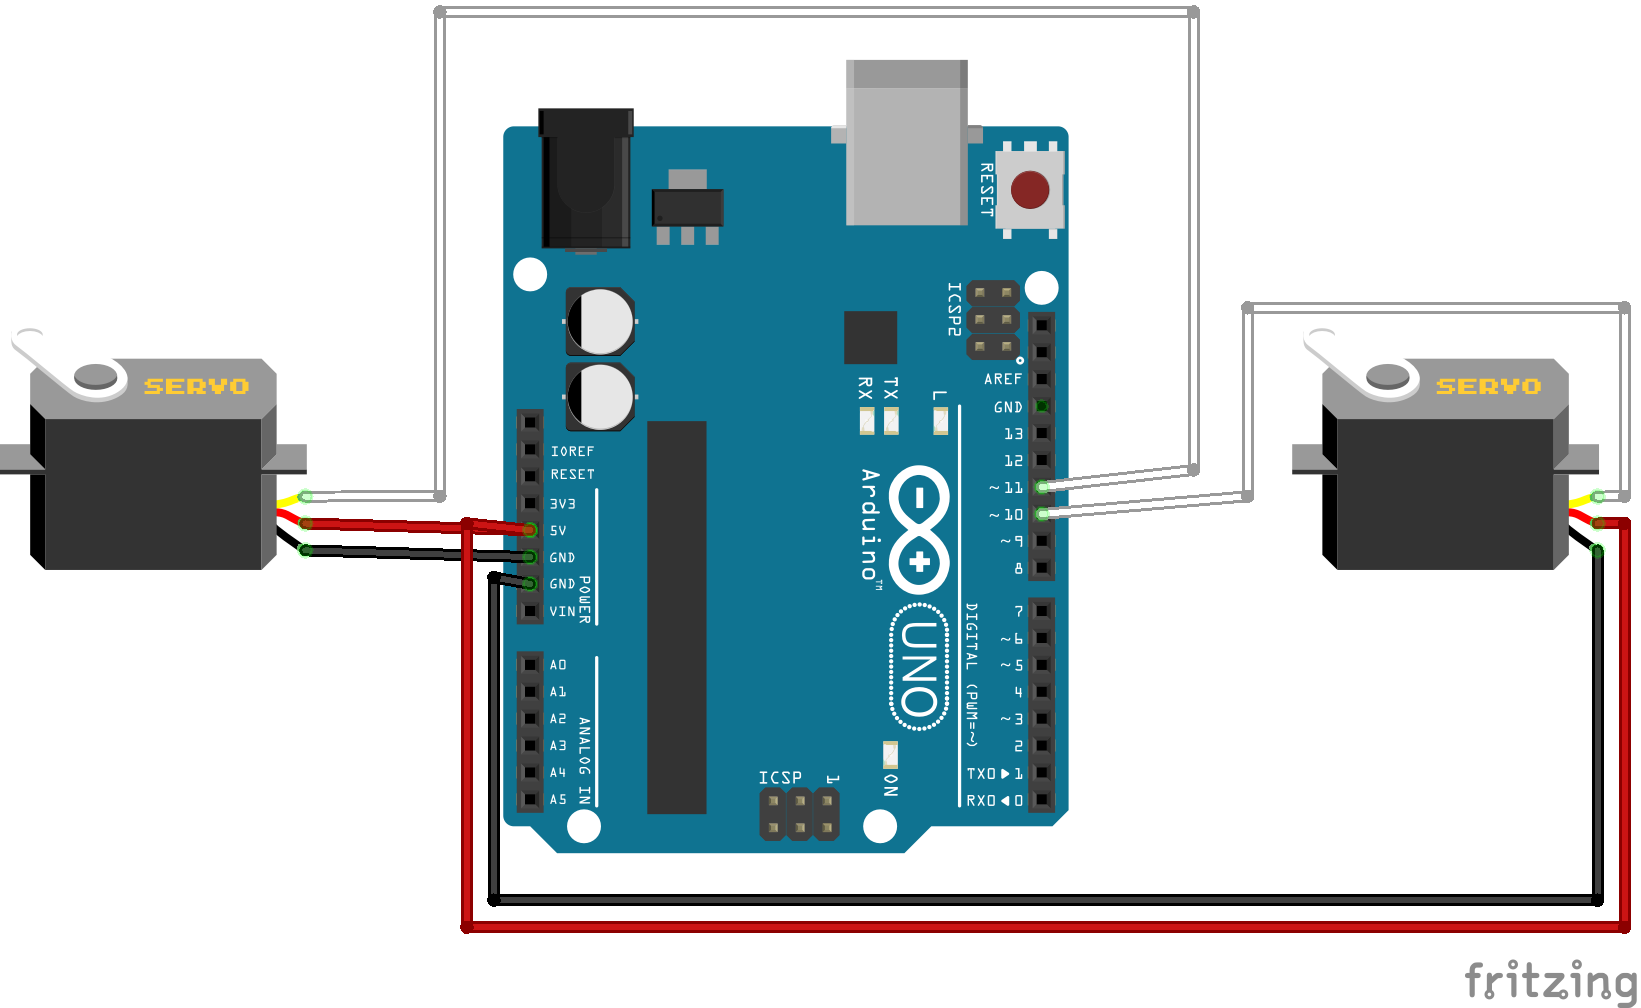
\includegraphics[width=\textwidth]{wiring.png}
    \caption{robot ciruit connections}
    \label{fig:circuit}
\end{figure}

Once you have made all your connections, you're ready to start programming.


\clearpage

\lstinputlisting{basic.ino}

\end{document}
